% !TEX root = diplomarbeit.tex
\chapter{Kommunikation Applikation und Hexacopter}
\renewcommand{\kapitelautor}{Autor: Katharina Joksch, Lucas Ullrich}
Um zwischen dem Hexacopter und dem Server eine Verbindung herzustellen wird eine Kommunikationsschnittstelle benötigt. Diese muss Drahtlos arbeiten und einen größeren Bereich
abdecken. Über diese werden anschließend die diversen Daten übertragen, dazu zählen \zB die Route, \bzw der Name des Gastes.

%%%%%%%%%%%%%%%%%%%%%%%%%%%%%%%%%%%%%%%%%%%%%%%%%%%%%%%%%%%%%%%%%%%%%%%%%%%%%%%
\section{Allgemeine technische Planung}
In der Planung wurde eine unkomplizierte und verlässliche Lösung für beide Kommunikationspartner gesucht. Da Bluetooth kaum noch standardmäßig verbaut wird hier wiederum
Serverseitig eine externe Hardware benötigt, um dies zu vermeiden wurde WLAN ins Auge gefasst.

WLAN stellte sich folglich als ideale Schnittstelle heraus,
es gibt die Möglichkeit zu Handover in sehr großen Bereichen, es ist nach einmaligem Setup vergleichsweise unkompliziert und es bietet diverse Möglichkeiten um festzustellen
ob die Verbindung noch aufrecht ist.

%%%%%%%%%%%%%%%%%%%%%%%%%%%%%%%%%%%%%%%%%%%%%%%%%%%%%%%%%%%%%%%%%%%%%%%%%%%%%%%
\section{Schnittstelle Hexacopter}
Seitens des Hexacopters wird ein zusätzliches Modul benötigt, dieses muss über eine der Schnittstellen des Mikrocontrollers ansprechbar sein.

  \subsection{Technische Planung}
  Bei der Planung wurde darauf geachtet ein WLAN-Modul zu wählen welches bekannter maßen funktioniert \bzw ein entsprechender Support zur Verfügung steht.
  So fiel die Wahl auf das WLAN-Modul RN171, vertrieben durch Microchip, hergestellt von Roving Networks.

  Das gewählte WLAN-Modul wird über eine UART-Schnittstelle angesteuert und verfügt über einige frei konfigurierbare Pins, diese werden schließlich zum Überwachen der
  Verbindung verwendet.

  \subsection{Umsetzung}
  Bei der Umsetzung stand für die anfänglichen Tests ein Evaluation-Kit zur Verfügung. Dieses kann ohne weitere Hardware direkt über ein USB-Kabel mit einem PC verbunden werden.
  So ist es möglich die nötigen Konfigurationen des Moduls auszutesten bevor dieses in der Hardware implementiert wird.

  \begin{figure}[H]
    \begin{centering}
      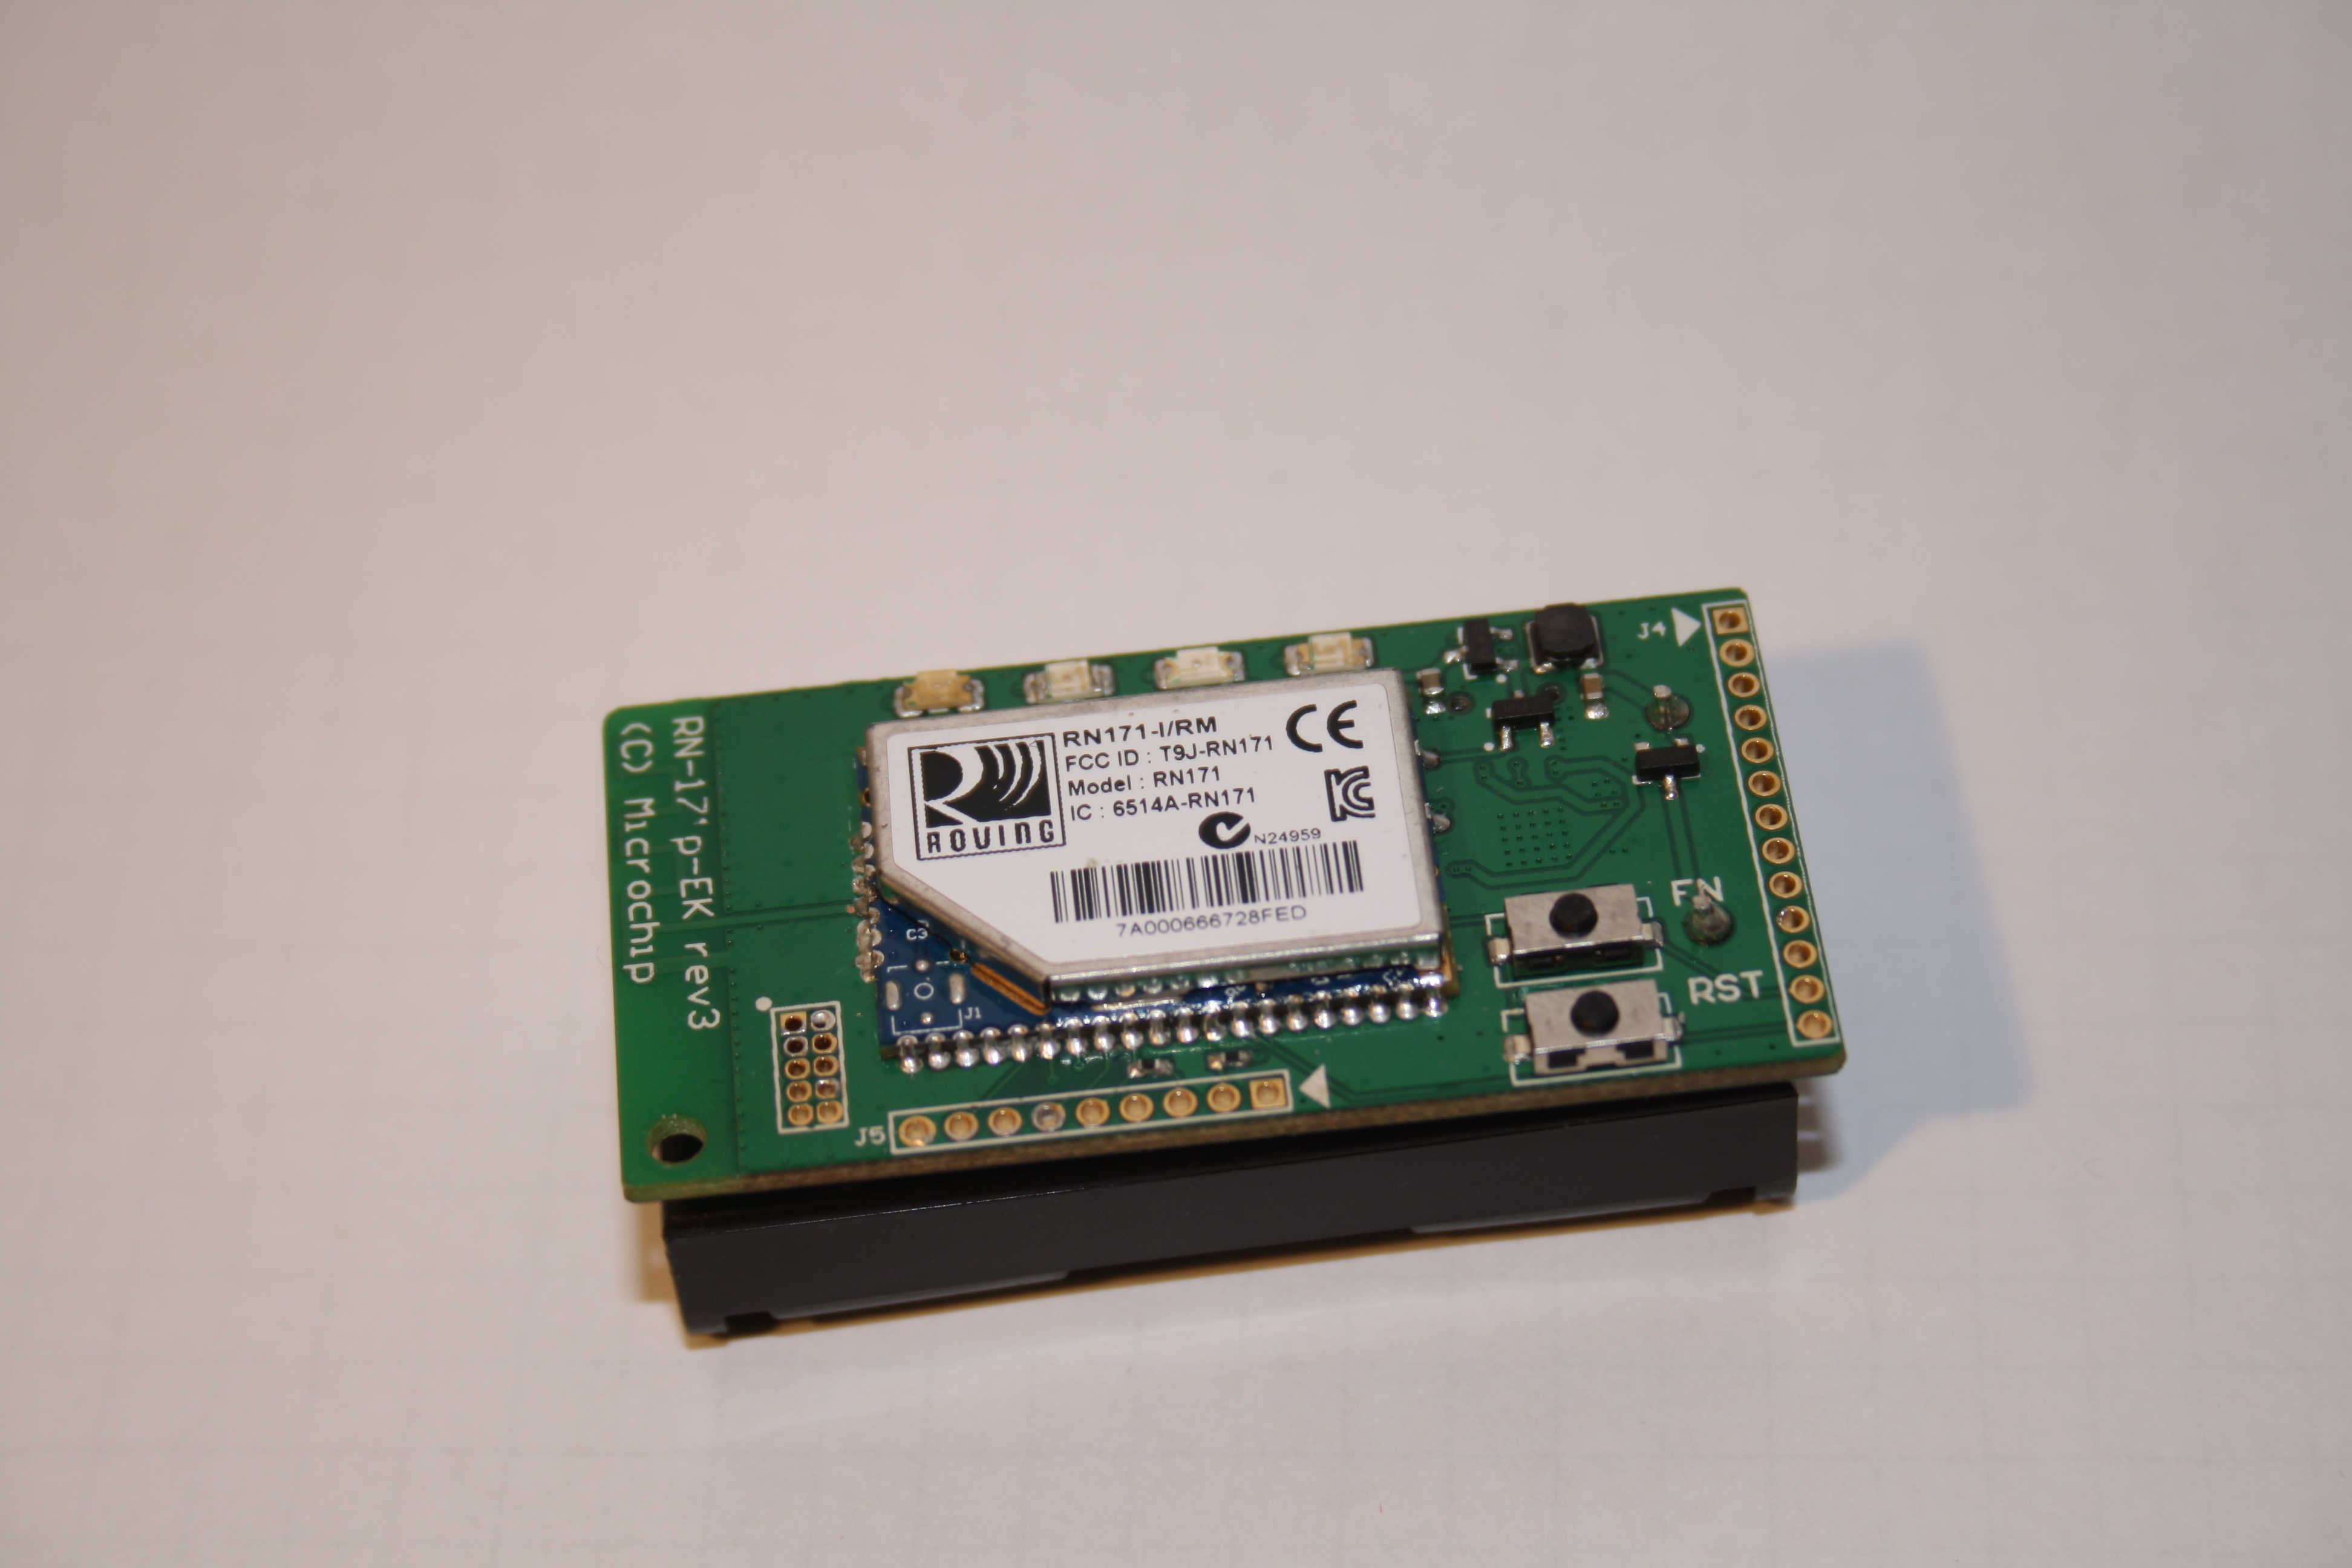
\includegraphics[width = 0.6\textwidth]{Bilder/RN171_EK}
    \par\end{centering}
    \caption[RN171 Evaluation-Kit]{RN171 Evaluation-Kit\cite{RN171_EK_source}}
    \label{RN171_EK}
  \end{figure}

  Um das WLAN-Modul so einzustellen, dass es sich Pin-gesteuert mit einem Host verbindet sind einige Schritte notwendig:
  \begin{itemize}
    \item \textbf{\$\$\$}\\
    Öffnet den Commandmode, nun können die Einstellungen vorgenommen werden
    \item \textbf{set wlan ssid <network\_name>}\\
    Deklariert den Netzwerknamen
    \item \textbf{set wlan phrase <network\_passphrase>}\\
    Deklariert das Passwort mit dem das Netzwerk gesichert ist
    \item \textbf{set ip host <host\_ip-address>}\\
    Deklariert die IP-Adresse des Empfängers
    \item \textbf{set ip remote <host\_portnumber>}\\
    Deklariert den Port auf dem der Empfänger die Daten empfangen soll
    \item \textbf{set sys iofunc 0x70}\\
    Durch diese Einstellung kann das WLAN-Modul über die Pins gesteuert werden
    \item \textbf{set wlan join 1}\\
    Stellt das WLAN-Modul auf automatisches Verbinden mit dem angegebenen Netzwerk ein
    \item \textbf{set ip protocol 4}\\
    Stellt das WLAN-Modul auf eine TCP/IP-Verbindung ein bei der nur Daten vom gespeicherten Host akzeptiert werden
    \item \textbf{set uart baud <desired-baudrate>}\\
    Stellt die Baudrate des WLAN-Moduls ein, Standard ist 9600
    \item \textbf{save}\\
    Speichert die Parameter in den Standardeinstellungen die nach einem Neustart geladen werden
    \item \textbf{reboot}\\
    Erzeugt einen Neustart bei dem die Standardeinstellungen geladen werden
  \end{itemize}
  Nachdem das WLAN-Modul auf die nötigen Parameter eingestellt ist, kann es direkt mit dem Mirkocontroller verbunden werden, die Verbidnung kann über einzelne Pins kontrolliert
  werden.

  \subsection{Herausforderungen und Lösungen}
  Eine Herausforderung stellte die Frage dar wie genau die Verbindung hergstellt wird. Das Datenblatt des WLAN-Moduls mit über 100 Seiten bietet viele potentielle Möglichkeiten.
  Die erste Wahl fiel auf das Auslesen einer Website, auf den ersten Anblick funktionierte das auch, jedoch musste festgestellt werden, dass unabhängig von der Website sehr ähnliche
  Daten verarbeitet werden, jedoch nicht der eigentliche Inhalt der Website sondern Providerinformationen.

  Die zweite Wahl fiel auf eine TCP/IP Verbindung, lediglich die genaue Umsetzung dieser ließ viele Möglichkeiten offen. Einerseits besteht die Möglichkeit eine Verbindung direkt
  über die Eingabe "open" im Commandmode zu öffnen, andererseits jedoch auch über die Pins als auch automatische Timeouts.

  Aufgrund der Einfachheit und vollen Kontrolle viel die Wahl auf die Ansteuerung über die Pins.
  Dazu stehen 3 unterschiedliche Pins zur Verfügung:
  \begin{itemize}
    \item \textbf{Associated}\\
    Mit einem Netzwerk verbunden
    \item \textbf{Open TCP connection}\\
    Die Verbidnung zum Host herstellen
    \item \textbf{Connected}\\
    Die Verbindung zum Host ist hergestellt
  \end{itemize}
  Die Statusinformationen Associated als auch Connected werden von dem WLAN-Modul geliefert, die Anweisung eine Verbindung herzustellen von dem Mirkocontroller.

%%%%%%%%%%%%%%%%%%%%%%%%%%%%%%%%%%%%%%%%%%%%%%%%%%%%%%%%%%%%%%%%%%%%%%%%%%%%%%%
\section{Schnittstelle Applikation}

  \subsection{Technische Planung}
  
      \subsubsection{Eclipse}
    
Eclipse ist eine freie Entwicklungsumgebung für Programme und wurde von der Eclipse Foundation entwickelt. Das Programm kann verwendet werden, um in mehreren Programmiersprachen Software zu entwicklen. Besonders gut geeignet ist Eclipse für die Entwicklung von Java-Programmen, da es sowohl Auto-Completion ermöglicht als auch Syntax- Highlighting.

	   \subsubsection{JDBC}

Die Java Datenbankschnittstelle JDBC ist ein Industriestandard für datenbankunabhängige Verbindungen zwischen Java Programmen, SQL Datenbanken und sämtlichen anderen tabellenbasierten Datenbankmodellen. Zu den Aufgaben von JDBC gehört es, Datenbankverbindungen aufzubauen und diese zu verwalten. Außerdem kann JDBC  SQL-Anfragen an die Datenbank weiterleiten, Ergebnisse in eine für Java nutzbare Form umwandeln und diese dem Programm zur Verfügung stellen.

	   \subsubsection{Zusammenspiel mit der Applikation und dem WLAN-Modul}
Das Java-Programm und die Applikation kommunizieren nur indirekt miteinander, da beide nur auf die Datenbank zugreifen um deren Inhalt zu überprüfen und Einträge updaten beziehungsweise erstellen.
Mit dem WLAN-Modul wird hingegen auf direktem Weg kommuniziert. Dieses wird nämlich als Thread etabliert und direkt in den Javaklassen verwaltet.
(Bild Aufbau)
  \subsection{Umsetzung}
Für die Umsetzung des Javaprogramms wurden drei verschiedene Klassen erstellt:
\begin{itemize}
    \item \textbf{SQL Reader}\\
Diese Klasse wurde dazu programmiert, alle Datenbankzugriffe zu regeln.
Um den Zugriff auf Datenbanken zu bewerkstelligen wurde JDBC verwendet. 
Damit das Programm mit JDBC arbeiten kann muss man es erst einmal von Oracle downloaden und anschließend mit einem Rechtsklick auf das Javaprojekt unter dem Menüpunkt "Properties" als Bibliothek angeben.
Wie auch bei Doctrine müssen der Datenbank Host, der Datenbank Port und die Benutzerdaten angegeben werden, damit die Verbindung hergestellt werden kann.
Als Treiber wird hier jedoch statt MySQL auf JDBC verwiesen. 
Um die Verbindung herzustellen wurde auf die Funktion DriverManager.getConnection() aufgerufen. Als Parameter musste ihr der Pfad zur Datenbank und die Benutzerdaten mitgeschickt werden.
\\
Damit die Tischdaten angezeigt werden konnten, wurde die "showTischdaten()"-Funktion erstellt. Um die ID, die Tischroute und die Tischnummer zu erhalten musste jeweils ein SQL-Statement, welches die Tischdaten ausliest, denen die Bestellung zugewiesen ist, verfasst werden, welches anschließend ausgeführt wurde.
Die Ergebnisse wurden in ein ResultSet gespeichert. Danach wurden sie in einer Schleife iteriert wurden und der aktuelle Wert aus dem ResultSet als String umgewandelt. Nun konnte die Route als Rückgabewert angegeben werden. Damit in der Bestellungen-Tabelle angemerkt wird, wann die Bestellung ausgeliefert wurde, wurde mit SQL ein Update-Statement erzeugt und mit der "executeUpdate()"-Funktion ausgeführt.
\\
Um in einer extra Datenbanktabelle den Verbindungsstatus zwischen dem Hexacopter und dem Server überprüfen zu können, wurde bei jeder Statusänderung die "erstelleDBEintrag()"-Funktion aufgerufen. Das Einfügen von Datenbankeinträgen kann mit einem Insert-Statement erledigt werden. Dieses muss im Anschluss ebenfalls mit der "executeUpdate()"-Methode durchgeführt werden.
    \item \textbf{Komm Manager}\\
Um die Threads zu managen wurde eine die "Komm Manager" Klasse programmiert.
Damit diese Klasse die Funktionen der "SQL Reader"-Klasse verwenden kann, erbt sie von dieser. Dies wird ganz oben bei der Klassendefinierung mithilfe dem Befehl "extends" gehandhabt. 
Als globale Variable wird ein Hashset, welches die Teilnehmer beeinhaltet, erstellt. 
Anschließend wird ein Server Socket erstellt, welchem später ein geeigneter Port zugewiesen wurde.
Mithilfe eines Timers wird regelmäßig überprüft ob ein Teilnehmer vorhanden ist. Wenn das der Fall ist, wird auf eine  Methode verwiesen, in welcher die Verbindung hergestellt wird und daher auch die SQl Readerfunktion aufgerufen wird, welche den Verbindungsstatus erneuert. Außerdem bekommt der Teilnehmer daraufhin durchgehend eine Nachricht zugeschickt.
Um zu überprüfen ob der Hexacopter in der Basis ist und somit bereit dazu ist eine Speise auszuliefern, wartet der Server darauf, dass im eine bestimmte Nachricht geschickt wird. Sobald diese bestimmte Nachricht ankommt, liefert die Funktion "true" zurück.
    \item \textbf{Komm Teilnehmer}\\
Die "Komm Teilnehmer" Klasse wurde dafür entwickelt, die einzelnen Verbindungen zum Hexacopter zu verwalten.
Dem Teilnehmer Thread wird sowohl der Manager als auch der Server Socket als Parameter mitgeliefert. Über diese kann im Anschluss das Senden und Empfangen der Nachrichten geregelt werden. 
In dieser Klasse wird die Nachricht des Hexacopters an die Manager Funktion geschickt, welche überprüft ob die Nachricht aussagt, dass sich der Multicopter in der Basis befindet. Wenn das der Fall ist, wird automatisch die Tischnummer der auszuliefernden Bestellung an den Teilnehmer geschickt.
  \end{itemize}

  \subsection{Herausforderungen und Lösungen}
verbundenstatus